%************************************************
\chapter{Dark sector phase transitions} \label{chp:pt}
%************************************************

\begin{flushright}
	\slshape
	It cannot be seen, cannot be felt,\\
	Cannot be heard, cannot be smelt,\\
	It lies behind stars and under hills,\\
	And empty holes it fills.\\ \medskip
	--- \textsc{Gollum}
\end{flushright}



In the previous two chapters we have introduced the field of \ac{GW} cosmology and reviewed the state of \ac{PTA} searches for stochastic \acp{GWB}. Now, we will go beyond the established  \ac{LCDM} expansion history and beyond \ac{SM} physics by studying \acp{FOPT} in the early universe. As we have seen in the introductory section~\ref{sec:chronology} on the chronology of the early cosmos, the history of our universe can be understood as a history of subsequent \acp{PT}: \graffito{Adding a dark \ac{PT} to the series of \ac{SM} ones} during inflation, a scalar field slowly rolled to obtain a new \ac{vev}. During reheating the equation of state of the Universe then changed from vacuum to radiation, corresponding to yet another \ac{PT}. It followed the \ac{EWPT}, as well as chiral symmetry breaking and confinement during the \ac{QCD} \ac{PT}. As we will show below, \acp{PT} are a generic feature of \acp{QFT} at finite temperature. This principle also applies to additional gauge groups extending the \ac{SM} of particle physics: as noted in section~\ref{sec:lcdmpuzzles}, only 15\% of the total non-relativistic matter in our Universe is accounted for by the \ac{SM} particle content. The remaining 85\% of matter motivate us to study the spontaneous breaking of a \textit{dark} symmetry group in this chapter.

In the following section~\ref{sec:finite-temp} we first make an analogy to a simple quantum mechanical harmonic oscillator coupled to a thermal bath to get an intuition for how a quantum field behaves at finite temperature. \graffito{Summary of this chapter} What follows is a discussion of the effective potential and the thermodynamics of \acp{FOPT} in the early universe in section~\ref{sec:fopts}. In section~\ref{sec:gwfopt} we then come to the prediction of \acp{GWB} from \acp{PT} in \acp{DS}.

\section{Finite-temperature effects in QFT} \label{sec:finite-temp}
\subsection{A quantum harmonic oscillator in a thermal bath}

To start our discussion of thermal field theory, we will begin with the conceptually much easier case of a quantum mechanical harmonic oscillator with Hamiltonian $\mathcal{H}$, the trace of which defines the partition function $Z(T) \equiv \text{Tr}\bb{\mathrm{e}^{- \beta \mathcal{H}}}$. Here and in the following, $\beta = T^{-1}$ denotes the inverse temperature of the bath to which the harmonic oscillator (and later the \ac{QFT}) is coupled. For a frequency $\omega$ of the oscillator, we obtain the partition function~\cite{Hindmarsh:2020hop}
\begin{align}
	Z_{\text{ho}} &= \begin{cases}
		\sum_{n = 0}^{\infty} \exp \bb{- \beta \omega \ba{n + \frac{1}{2}}} = \mathrm{e}^{- \beta \omega /2} \ba{1 - \mathrm{e}^{- \beta \omega}}^{-1}\\
		\sum_{n = 0}^{1} \exp \bb{- \beta \omega \ba{n + \frac{1}{2}}} = \mathrm{e}^{\beta  \omega /2}  \ba{1 + \mathrm{e}^{- \beta \omega / 2}},
	\end{cases}
\end{align}
where the above (below) expression holds for a bosonic (fermionic) oscillator. One can show that a system in thermal equilibrium will eventually go to a state with minimal free energy $F	 \equiv - T \ln Z(T)$. For the above partition function of a harmonic oscillator, we obtain
\begin{align}
	F_{\text{ho}} = \begin{cases}
		\frac{\omega}{2} + T \ln \ba{1 - \mathrm{e}^{-\beta \omega}} &\text{for bosons}\\
		-\frac{\omega}{2} - T \ln \ba{1 + \mathrm{e}^{-\beta \omega}} &\text{for fermions} .
	\end{cases} \label{eq:FE_ho}
\end{align}
This is already the result which we wanted to obtain in this brief section: the free energy of a single harmonic oscillator is the sum of a temperature-independent term corresponding to the ground state energy $\hbar \omega/2$ and a temperature-dependent \graffito{The free energy of a harmonic oscillator} term which accounts for the occupation of higher states due to the available thermal energy. The first term is purely quantum mechanical and corresponds to Heisenberg's uncertainty in the oscillator's position and momentum, whereas the second term instead arises due to the coupled thermal bath and dominates the free energy for sufficiently high temperatures. Indeed, we will recover a remarkably similar expression after a much more tedious computation for the case of \ac{QFT} coupled to a thermal bath.

\subsection{The Kubo-Martin-Schwinger relation}
We now want to transition from quantum mechanics to \ac{QFT}. To do so, let us repeat that in statistical mechanics the expectation value of a given operator $A$ is given by the thermally averaged sum of $A$ over eigenstates of the Hamiltonian $\mathcal{H}$,
\begin{align}
	\langle A \rangle_\text{T} \equiv \frac{1}{Z} \text{Tr}\bb{\mathrm{e}^{- \beta \mathcal{H}} A}  .
\end{align}
In particular, this also holds for the correlators of quantum fields $\phi$. To obtain the famous Kubo-Martin-Schwinger relation~\cite{Kubo:1957mj,Martin:1959jp}, consider the two-point function of a quantum field $\phi_{\bm{y}}$ at position $\bm{y}$ at time $t$ and the field at position $\bm{x}$ at zero time, 
\begin{align}
	\langle \phi_{\bm{y}}(t) \phi_{\bm{x}}(0) \rangle_\text{T} &= \frac{1}{Z} \text{Tr} \bb{\mathrm{e}^{- \beta \mathcal{H}}  \phi_{\bm{y}}(t) \phi_{\bm{x}}(0) } \nonumber\\
	&= \frac{1}{Z} \text{Tr} \bb{\phi_{\bm{y}}(t)   \mathrm{e}^{-\beta \mathcal{H}} \mathrm{e}^{\mathrm{i} (-\mathrm{i} \beta \mathcal{H})}  \phi_{\bm{x}}(0)  \mathrm{e}^{-\mathrm{i} (-\mathrm{i}\beta \mathcal{H})} } \nonumber\\
	&= \frac{1}{Z} \text{Tr} \bb{ \phi_{\bm{y}}(t)  \mathrm{e}^{- \beta \mathcal{H}}  \phi_{\bm{x}}(- \mathrm{i} \beta) } \nonumber\\
	&= \frac{1}{Z} \text{Tr} \bb{\mathrm{e}^{- \beta\mathcal{H}} \phi_{\bm{x}}(- \mathrm{i} \beta)  \phi_{\bm{y}}(t) } \nonumber\\
	&= \langle \phi_{\bm{x}}(- \mathrm{i} \beta)  \phi_{\bm{y}}(t) \rangle_\text{T} \nonumber\\
	&= \pm \langle \phi_{\bm{y}}(t)  \phi_{\bm{x}}(- \mathrm{i} \beta) \rangle_\text{T} \, . \label{eq:KMS}
\end{align}
To arrive at the final expression we made repeated use of the permutation rule for traces and employed the time evolution $\phi_{\bm{x}}(t) = \mathrm{e}^{\mathrm{i} \mathcal{H} t} \phi_{\bm{x}}(0) e^{-\mathrm{i} \mathcal{H} t}$. In the last step, a minus sign occurs only for fermionic fields due to them anti-commuting, but not for bosonic fields. We can hence see that \graffito{The emergence of periodicity in imaginary time} a bosonic (fermionic) field $\phi$ needs to be symmetric (anti-symmetric) and cyclic in time with the periodicity $- \mathrm{i} \beta$ if it is coupled to a thermal bath with inverse temperature $\beta$.

We now go to \textit{purely} imaginary time $t \rightarrow \tau = - \mathrm{i} t$ by performing a Wick rotation. We find that in the so-called imaginary-time (or Matsubara) formalism, the Euclidean time parameter $\tau$ can be identified with the inverse temperature $\beta$~\cite{Matsubara:1955ws}. In performing the Wick rotation, we gained access to the description of systems in thermal equilibrium, but lost control over dynamical processes happening in real time. In the alternative, more involved real-time (or Keldysh)  formalism~\cite{Keldysh:1964ud} both is possible simultaneously, thus allowing the description of out-of-equilibrium dynamics. For our goal of identifying the phase structure of a given \ac{QFT}, the Matsubara formalism is sufficient, however. To \graffito{Matsubara sums} go from correlators in a \ac{QFT} at zero temperature to those of a finite-temperature \ac{QFT}, we therefore need to replace the integral over the time component in the occurring integrals over Euclidean four-momentum space $k_\text{E}^\mu = \ba{k_\text{E}^0, \bm{k}_\text{E}}$ with a discrete sum over the so-called Matsubara frequencies $k_\text{E}^0 = \omega_n$~\cite{Quiros:1999jp},
\begin{align}
	&\int \frac{\diff^4 k_\text{E}}{\ba{2 \pi}^4} f(k_\text{E}) \rightarrow T \sum_{n = - \infty}^\infty \int \frac{\diff^3 k}{\ba{2 \pi}^3} f(\omega_n, \mathbf{k})
	\label{eq:TFT} \nonumber \\ 
	&\text{with} \qquad \omega_n = \begin{cases}
		2n \pi T &\text{for bosons}\\
		(2n + 1) \pi T &\text{for fermions} .
	\end{cases} 
\end{align}
The summation corresponds to the integration over time in the theory with $T=0$ and may be arbitrarily complicated for a general integrand. Intuitively, the Matsubara sum adds up all contributions to a given integral allowed by the field boundary conditions set by the Kubo-Martin-Schwinger relation in equation~\eqref{eq:KMS}. 


\subsection{The effective potential of an abelian gauge theory}
\label{sec:VeffU1}

\paragraph{The tree-level potential} For discreteness, we now want to study the finite-temperature behavior of an additional dark $U(1)^\prime$ extending the gauge groups of the \ac{SM}. This model will be of \graffito{A dark $U(1)^\prime$ gauge symmetry} particular relevance in chapter~\ref{chp:LISA}. Its Lagrangian density is given by
\begin{align}
	\mathcal{L} &= \left|D_\mu \Phi \right|^2 - \frac{1}{4} B_{\mu \nu}B^{\mu \nu}  + \mu^2 \left|\Phi\right|^2 - \lambda \left|\Phi\right|^4 \nonumber\\
	&\quad + \chi_\text{L}^\dagger \mathrm{i} \slashed{D} \chi_\text{L} + \chi_\text{R}^\dagger \mathrm{i} \slashed{D} \chi_\text{R}  - y \Phi \chi_\text{L}^\dagger \chi_\text{R} - y \Phi^* \chi_\text{R}^\dagger \chi_\text{L} \, .
	\label{eq:toylagrangian}
\end{align}
The complex scalar field $\Phi$ and the chiral fermions $\chi_\text{L}$ and $\chi_\text{R}$ are charged under the $U(1)^\prime$ gauge group. Their $U(1)^\prime$ charges satisfy $Q_\Phi = Q_{ \chi_\text{L}} - Q_{ \chi_\text{L}}$, which we realize through the choice $Q_\Phi = 1$, $Q_{\chi_\text{L}}  = + 1/2$ and $Q_{\chi_\text{R}}= - 1/2$ in order to preserve the gauge symmetry of the Yukawa interaction term and keep the model free of anomalies. This choice allows us to express the interactions of the chiral fermions as those of a single Dirac bi-spinor field in the following. The field strength tensor is defined in terms of the dark photon field $A_\mu^\prime$ as $B_{\mu \nu} = \partial_\mu A^\prime_\nu - \partial_\nu A_\mu^\prime$ and the corresponding covariant derivative reads $D_\mu = \partial_\mu + \mathrm{i} g A^\prime_\mu$. In principle, also a  \graffito{We ignore portal couplings} mixing term $\propto \Phi^2 H^2$ with the \ac{SM} Higgs field $H$ and a kinetic mixing term $\propto F_\mn B^\mn$ with the \ac{SM} photon $F_\mn$ would be allowed. In order to be able to ignore their effects on the effective potential for simplicity, we assume the respective portal couplings to be sufficiently small~\cite{Ilten:2018crw,Bauer:2018onh, Ferber:2023iso}. We will revisit their effect in chapters~\ref{chp:ptabbn} and \ref{chp:LISA} when discussing the decay of \acp{DS} in order to satisfy cosmological constraints.

The above Lagrangian features the tree-level potential $V_\text{tree}(\Phi) = - \mu \abs{\Phi}^2 + \lambda \abs{\Phi}^4$, having a \graffito{Expanding around the tree-level minimum} $U(1)^\prime$-symmetric minimum at $\abs{\Phi}^2 = \mu^2 / \lambda$. At a given point in space, the field must be in a single vacuum state, whereas the above condition is satisfied by an infinite set of fields related by the gauge transformation $\Phi \rightarrow \mathrm{e}^{\mathrm{i} \alpha} \Phi$ with $\alpha \in \left[0, 2\pi \right)$. For convenience we choose the vacuum to lie on the real field axis, thus breaking the $U(1)^\prime$ spontaneously. Here, \textit{spontaneously} refers to the field direction with zero complex phase being arbitrary among the line of potential minima. Upon this choice, we can expand the Lagrangian around $\Phi = (\phi + v_\phi +  \mathrm{i} \varphi)/\sqrt{2}$ with $\phi$ and $\varphi$ being real fields and $v_\phi \equiv \mu / \sqrt{\lambda}$, eventually obtaining
\begin{align}
	\mathcal{L} &=  \frac{1}{2}\partial_\mu \phi \partial^\mu \phi + \frac{1}{2} \partial_\mu\varphi \partial^\mu\varphi - \frac{1}{4} A'_{\mu\nu}A^{'\mu\nu}
	- \frac{1}{2} m_\phi^2\phi^2 + \frac{1}{2}m_{A'}^2A^{'2}_\mu  \notag \\
	&\quad -gA'_\mu[\varphi\partial^\mu\phi - \phi\partial^\mu\varphi - v_{\phi}\partial^\mu\varphi] + \frac{g^2}{2}\phi^2A^{'2}_\mu + \frac{g^2}{2}\varphi^2 A^{'2}_\mu \nonumber \\
	&\quad  + g^2v_{\phi}\phi A^{'2}_\mu -\lambda v_{\phi}\phi^3 - \lambda v_{\phi}\varphi^2\phi - \frac{\lambda}{4}\phi^2\varphi^2 - \frac{\lambda}{4}\phi^4 -\frac{\lambda}{4} \varphi^4\notag\\
	&\quad  +\mathrm{i}\bar\chi\slashed{\partial}\chi - m_\chi\bar\chi\chi + \frac{g}{2}\bar\chi\slashed{A}'\gamma^5\chi -
	\frac{y}{\sqrt{2}}\phi\bar\chi\chi + \mathrm{i}\frac{y}{\sqrt{2}}\varphi\bar\chi\gamma^5\chi 
\end{align}
with the tree-level masses
\begin{subequations}
	\begin{align}
		m_\phi^2 &= 3 \lambda v_\phi^2 - \mu^2 = 2 \lambda v_\phi^2 \, , &  {m_{A^\prime}}^2 &= g^2 v_\phi^2 \, , \\
		m_\varphi^2 &= \lambda v_\phi^2 - \mu^2 = 0 \, ,
		 &\text{and} \qquad \qquad m_\chi^2 &= \frac{y^2 v_\phi^2}{2} \, .
		 \label{eq:masses}
	\end{align}
\end{subequations}


\paragraph{Including quantum effects} The above mass spectrum only holds at tree-level, i.e.~in the limit $\hbar \rightarrow0$. Due to $\Phi$ being a quantum field, however, quantum corrections become relevant for non-zero field values. Mathematically, the effect of quantum corrections can be included by  promoting the tree-level potential $V_\text{tree}$ in eq.~\eqref{eq:toylagrangian} to a so-called effective potential. The effective potential contribution of $\ell$-loop Feynman diagrams, corresponding to an expansion in powers of $\hbar^\ell$, can be derived using the path-integral formulation of \ac{QFT} and reads~\cite{Weinberg:1996kr}
\begin{align}
	V_{\text{eff}}^{\ell}(\phi) = - \sum_{k=0}^{\infty} \frac{\phi^k}{k!} \, \Gamma^{(k)}_\ell (p=0) \, .
\end{align}
Here, $\Gamma^{(k)}_\ell$  is the $k$-point, $\ell$-loop effective vertex with all external momenta set to zero. Ignoring loop diagrams ($\ell = 0$), one therefore \graffito{The one-loop order} just recovers the tree-level potential. At leading loop order $(\ell = 1)$ and only considering $\Phi$-loops, we instead obtain the sum
\begin{align}
	V_{\text{eff}, \Phi}^1(\phi) &=
	\bb{\phi^2 \, 
		\vcenter{\hbox{\begin{tikzpicture} 
					\draw[thick,insert vertex=0] (0,0) arc(360:0:0.4);
					\draw[thick,dashed] (0.2, 0.4) -- (0,0) -- (0.2, -0.4);
		\end{tikzpicture}}}
		+\phi^4 \, 
		\vcenter{\hbox{\begin{tikzpicture} 
					\draw[thick,insert vertex/.list={0,0.5}](0,0) arc(360:0:0.4);
					\draw (0,0) arc(360:0:0.4);
					\draw[thick,dashed] (0.2, 0.4) -- (0,0) -- (0.2, -0.4);
					\draw[thick,dashed] (-1, 0.4) -- (-0.8,0) -- (-1, -0.4);
		\end{tikzpicture}}}
		+\phi^6 \,
		\vcenter{\hbox{\begin{tikzpicture} 
					\draw[thick,insert vertex/.list={0,1/3,2/3}](0,0) arc(360:0:0.4);
					\draw (0,0) arc(360:0:0.4);
					\draw[thick,dashed] (0.2, 0.4) -- (0,0) -- (0.2, -0.4);
					\draw[thick,dashed] (-1.05, 0.32) -- (-0.6, 0.35) -- (-0.36, 0.72);
					\draw[thick,dashed] (-1.05, -0.32) -- (-0.6, -0.35) -- (-0.36, -0.72);
		\end{tikzpicture}}}+\dots}_{p=0} \nonumber \\
	&= 2 \mathrm{i} \sum_{n = 1}^{\infty} \int\frac{\diff^4 k}{\ba{2 \pi}^4} \frac{1}{2n} \bb{\frac{6 \lambda \phi^2 / 2}{k^2 + \mu^2 + \mathrm{i} \epsilon}}^n  .
	\label{eq:UVdivergence}
\end{align}
In the above diagrams we denote the real part $\phi$ of the Higgs field with dashed lines, whereas solid lines refer to $\Phi$ comprising both the imaginary and real field components. In the second step we used that the $n$-th diagram has $2n$ external legs and $n$ propagators. Additionally, there are symmetry factors of $1/(2n)$ and $1/2^n$ from cyclic and anti-cyclic permutations of the vertices as well as permutations of the external lines of each vertex, respectively. The initial factor 2 accounts for the two internal \acp{dof} of $\Phi$ on the loop. Further, we used that each vertex comes with a factor $-6\mathrm{i}\lambda$ and each internal propagator brings a factor $\mathrm{i} / (k^2 + \mu^2 + \mathrm{i} \epsilon)$.

We can perform the sum over $n$ by comparing with the series expansion of $\ln(1+x)$ around $x=0$. Further performing a Wick rotation we arrive at
\begin{align}
	V_{\text{eff}, \Phi}^1(\phi) = \int \frac{\diff^4 k_\text{E}}{\ba{2  \pi}^4} \ln \bb{k_{\text{E}}^2 + m^2_\phi(\phi)} .
\end{align}
So far we only considered the effect of quantum corrections arising due to the self-coupling $\lambda$ of $\Phi$ to $\phi$, but not the effect of the gauge boson $A$ and the fermion $\chi$. One can show that also fermions and \graffito{Contributions from all charged fields} gauge bosons contribute in a similar way to the effective potential through their loop contributions, up to a factor corresponding to their \acp{dof} and a respective sign $\eta_a = +1$ $(-1)$ for bosons (fermions)~\cite{Quiros:1999jp}:
\begin{align}
	V_\text{eff}^1(\phi) = \sum_a \frac{\eta_a n_a}{2} \int \frac{\diff^4 k_\text{E}}{\ba{2  \pi}^4} \ln \bb{k_\text{E}^2 + m^2_a(\phi)}  .
\end{align}
Here, the sum goes over all particle species $a$ coupled to $\phi$, with $n_a$ being their internal \acp{dof}.


\paragraph{Going to finite temperature} To now compute the effective potential at finite temperature $T_\text{d} = \xi T$ (with the index d indicating a potential mismatch $\xi$ between the \ac{DS} temperature and the visible sector temperature $T$), we make use of the replacement rule from eq.~\eqref{eq:TFT} and obtain
\begin{align}
	V_\text{eff}^1(\phi, T_\text{d}) &= \sum_a \frac{\eta_a n_a T_\text{d}}{2} \sum_n \int \frac{\diff^3 k}{\ba{2  \pi}^3} \ln \bb{\omega_n^2 + k^2 + m^2_a} \nonumber\\
	&= \sum_a \eta_a n_a  \int \frac{\diff^3 k}{\ba{2 \pi}^3} \bb{\frac{E_a}{2} + T_\text{d} \ln \ba{1 - \eta_a \mathrm{e}^{- E_a /T_\mathrm{d}}}} \nonumber\\
	&= V_\text{CW}(\phi) + V_\text{T}(\phi, T_\text{d})  \, .
	\label{eq:Veffbeforereno}
\end{align}
To simplify the notation, the energy parameter $E_a^2 \equiv k^2 + m^2_a$ was introduced.  What we retrieve, closely resembles the free energy of a single harmonic oscillator which we derived in eq.~\eqref{eq:FE_ho}. Now, \graffito{The harmonic oscillator is everywhere} however, the frequency $\omega$ of the oscillator corresponds to a quantum field's energy $E_a$, which is integrated over. This is analogous to the naive image of a quantum field to be a superposition of infinitely many harmonic oscillators at each point in space. We obtained both a temperature-dependent and temperature-independent part, the latter of which corresponds to the (yet unrenormalized) Coleman-Weinberg potential~\cite{Coleman:1973jx}. 

The temperature-dependent part can be expressed as
\begin{align}
	V_\text{T}(\phi, T_\text{d})& = \frac{T^4_\text{d}}{2  \pi^2} \sum_a \eta_a  n_a  J_{\eta_a}\ba{\frac{m_a^2(\phi)}{T^2_\text{d}}} \quad \text{with} \\
	J_{\eta_a}\ba{z^2} &\equiv \int_{0}^{\infty} \diff y \,  y^2 \ln \bb{1 - \eta_a  \exp \ba{- \sqrt{y^2 + z^2}}} .
	\label{eq:thermalfunction}
\end{align}
Fig.~\ref{fig:thermalfunctions} shows the real part of the thermal functions $J$ in dependence of $z_a = m^2_\mathrm{a}/T_\mathrm{d}^2$.\footnote{The behavior of the thermal functions in fig.~\ref{fig:thermalfunctions} at negative $z^2$ is relevant as the scalar field will obtain an imaginary mass wherever the potential has a negative curvature. An in-depth study of the imaginary parts of the effective potential was performed in ref.~\cite{Delaunay:2007wb}. Generally speaking, an imaginary part of the effective potential indicates an instability of the vacuum at a specific field value, eventually triggering a \ac{PT}. } In the low-temperature limit, $z \rightarrow \infty$, the thermal functions and therefore also $V_\text{T}$ vanish. In the high-temperature limit, $z \rightarrow 0$, the thermal functions can instead by approximated by~\cite{Quiros:1999jp}
\begin{subequations}
	\label{eq:high-TJs}
	\begin{align}
		J_\text{bos}(z^2) &\approx - \frac{\pi^4}{45} + \frac{\pi^2}{12} z^2 - \frac{\pi}{6} z^3 - \frac{z^4}{32} \ln \ba{z^2} + \text{const}\, , \label{eq:high-TJbos}\\
		J_\text{ferm}(z^2) &\approx \frac{7 \pi^4}{360} - \frac{\pi^2}{24} z^2 - \frac{z^4}{32} \ln \ba{z^2} + \text{const}\, .
	\end{align}
\end{subequations}
The leading-order correction to the tree-level potential due to a single bosonic \ac{dof} hence reads $\pi^2 T^4_\text{d} /90$ if $T_\text{d} \gg m_a$, i.e.~the Stefan-Boltzmann law we already identified in eq.~\eqref{eq:rhorel}. \graffito{Interpreting the thermal corrections} Typically, this contribution to the vacuum energy density is absorbed into the cosmological constant, as it does not directly influence the dynamics of the scalar field. Note, however, in particular the $z^2$ terms in eqs.~\eqref{eq:high-TJs}, which translate to a term $V_\text{T}(\phi, T_\text{d}) \propto \phi^2 T^2_\text{d}$, acting as a temperature-dependent mass in the effective potential. At sufficiently high temperatures, these temperature-dependent mass terms inevitably  dominate over any other mass contribution, forcing the potential minimum to reside at vanishing field values $\phi = 0$. This phenomenon is known as symmetry restoration at high temperatures, if $\phi \neq 0$ refers to a phase in which a symmetry of the high-temperature \ac{QFT} is broken as in the present case of the spontaneous $U(1)^\prime$ breaking.

High-temperature symmetry restoration is a feature of many \acp{QFT} and the reason for us to understand the cosmic expansion history as a sequence of \acp{PT}: When temperature drops, the effect of $V_\text{T}$ decreases and the positions of the potential minima change. In fact it is not of further relevance if $\Phi$ is a fundamental scalar (as the \ac{SM} Higgs field triggering the \ac{EWPT}) or a bi-linear condensate $\langle \bar{q} q \rangle$ of fermions (like the quarks $q$ in the \ac{QCD} \ac{PT}). In the specific case \graffito{High-temperature symmetry restoration} of the tree-level potential $V_\text{tree} = - \mu^2 \phi^2 + \lambda \phi^4$, again considering only the $\phi^2$ term of the effective potential and ignoring $\mathcal{O}(1)$ factors, we see that at high temperatures it will effectively include a term that reads $V(\phi, T_\text{d}) \supset \ba{-\mu^2 + \lambda T_\text{d}^2} \phi^2$, indicating that for $T_\text{d} \lesssim \mu / \sqrt{\lambda}$ the $\phi = 0$ phase will become unstable.

\begin{figure}[t]
	\centering
	\includegraphics[width=\linewidth]{thesisplots/thermal_functions/thermal_functions}
	\caption{The real part of the thermal functions $J_\text{bos}(z^2)$ and $J_\text{ferm}(z^2)$.}
	\label{fig:thermalfunctions}
\end{figure}



\paragraph{The breakdown of perturbativity} The contributions $V_\text{CW}$ and $V_\text{T}$ to the effective potential can hence be regarded as corrections to the potential energy density of a scalar field $\phi$. However, both terms are still plagued by divergences. This is expected as eq.~\eqref{eq:UVdivergence} includes diagrams with two and four external legs for which the integrand is unbounded in the \ac{UV} limit of large loop momenta. But also the second, temperature-dependent term is expected to feature a breakdown of perturbativity by the mere existence of two energy scales, namely \graffito{\ac{UV} and \ac{IR} divergences} temperature and the scalar's mass~\cite{Curtin:2016urg}. The latter is an \ac{IR} divergence which can be understood by the thermal distribution of bosons $\bb{\exp\ba{E/T}-1}^{-1} \rightarrow T/E$ diverging for $T \gg E$: At high temperatures their distribution is dominated by low-energy bosons and diverges for soft bosons with $E \rightarrow 0$. This translates to an effective increase of the coupling between infrared bosons up to the point where the coupling between them becomes non-perturbative and our perturbative expansion breaks down.

The \ac{UV} divergence of the Coleman-Weinberg potential can be treated by dimensional regularization. Using the $\overline{\text{MS}}$ renormalization scheme we arrive at~\cite{Basler:2018cwe,Athron:2023xlk, Coleman:1973jx}
\begin{align}
	V_\text{CW}(\phi) = \sum_x \eta_x n_x \frac{m_x^4(\phi)}{64 \pi^2} \bb{\ln \frac{m_x^2(\phi)}{\Lambda^2}- C_x}
\end{align}
with $C_x$ being equal to $3/2$ ($5/6$) for scalars and fermions (gauge bosons) and $\Lambda$ being the renormalization scale~\cite{Basler:2018cwe,Athron:2023xlk, Quiros:1999jp}. To arrive at the above expression, the dimensionality of the integral in eq.~\eqref{eq:Veffbeforereno} was first formally shifted to $4 - \epsilon$. The singularities are then isolated in terms $\propto \epsilon^{-1}$, which need to be canceled by adding a finite counterterm potential $V_\text{ct}$~\cite{Quiros:1999jp}. In this thesis, we will impose the renormalization conditions $0 = \partial_\phi \left.\ba{V_\text{CW} + V_\text{ct}}\right|_{\phi = \Lambda}$ and $0 = \partial_\phi^2 \left.\ba{V_\text{CW} + V_\text{ct}}\right|_{\phi = \Lambda}$, effectively fixing the tree-level \ac{vev} and the Higgs mass $m_\phi$ to remain unchanged when going from tree-level to one-loop order, and set $\Lambda = v_\phi$.

\paragraph{Hard thermal loops} The divergences of the $T_\text{d}$-dependent term in eq.~\eqref{eq:Veffbeforereno} cannot be treated as simply: Consider for instance diagram (a) in fig.~\ref{fig:hardthermalloops}. Evaluating it by applying the replacement rule from eq.~\eqref{eq:TFT} for vanishing external momenta we obtain
\begin{align}
	\Pi_\phi(T_\text{d}) &= \lambda T_\text{d} \sum_n \int \frac{\diff^3 k}{\ba{2 \pi}^3} \frac{1}{\omega_n^2 + k^2 + m_\phi^2} \nonumber \\ &= \lambda  \int \frac{\diff^4 k}{\ba{2 \pi}^4} \ba{\frac{1}{2 E_\phi} + \frac{1}{E_\phi} \frac{1}{\mathrm{e}^{-E_\phi/T_\text{d}} - 1} } \overset{T \gg m_\phi}{\approx} \frac{\lambda T^2_\text{d}}{12}
\end{align}
In the last step we assumed that $T_\mathrm{d} \gg m_\phi$ and discarded the temperature-independent and \ac{UV}-divergent first term in brackets. In fig.~\ref{fig:hardthermalloops} the other one-loop corrections \graffito{Debye masses} for the scalar and gauge boson propagator of the Lagrangian in eq.~\eqref{eq:toylagrangian} are listed. These so-called Debye masses are generally of the form $\Pi_\phi \propto \lambda T_\text{d}^2$ for scalars and $\Pi_{A^\prime} \propto g^2 T_\text{d}^2$ for longitudinally polarized gauge bosons. We left out fermion Debye masses, since they will not appear in the effective potential at leading order, as we will show below.

\begin{figure}[t!]
	\myfloatalign
	\subfloat[]{$\vcenter{\hbox{\begin{tikzpicture} 
					\draw[thick,insert vertex=0] (0,0) arc(270:-90:0.4);
					\draw[thick,dashed] (-0.8, 0) -- (0,0) -- (0.8, 0);
		\end{tikzpicture}}} = 2 \cdot \pdd{m_\phi^2(\phi)}{\phi} \frac{T^2_\text{d}}{24} $} \quad
	\subfloat[]{$\vcenter{\hbox{\begin{tikzpicture} 
					\draw[thick,fermion arc arrow/.list={0.31,0.81}] (0,0) arc(360:0:0.4);
					\path[insert vertex/.list={0,0.5}](0,0) arc(360:0:0.4);
					\draw[thick,dashed] (0.8, 0) -- (0,0);
					\draw[thick,dashed] (-1.6, 0) -- (-0.8,0);
		\end{tikzpicture}}} = 4 \cdot \pdd{m_\chi^2(\phi)}{\phi} \frac{T^2_\text{d}}{48} $} \quad
	\subfloat[]{$\vcenter{\hbox{\begin{tikzpicture}
					\draw[gaugeboson] (0,0) arc(270:-90:0.4);
					\path[insert vertex=0] (0,0) arc(270:-90:0.4);
					\draw[thick,dashed] (-0.8, 0) -- (0,0) -- (0.8, 0);
		\end{tikzpicture}}}= 3 \cdot \pdd{m_{A^\prime}^2(\phi)}{\phi} \frac{T^2_\text{d}}{24} $} \quad
	\subfloat[]{$\vcenter{\hbox{\begin{tikzpicture} 
					\draw[thick,insert vertex=0] (0,0) arc(270:-90:0.4);
					\draw[gaugeboson] (-0.8, 0) -- (0,0) -- (0.8, 0);
		\end{tikzpicture}}} + \vcenter{\hbox{\begin{tikzpicture} 
					\draw[thick] (0,0) arc(360:0:0.4);
					\path[insert vertex/.list={0,0.5}](0,0) arc(360:0:0.4);
					\draw[gaugeboson] (0.8, 0) -- (0,0);
					\draw[gaugeboson] (-1.6, 0) -- (-0.8,0);
		\end{tikzpicture}}} =
		\begin{cases}
			2 \cdot \frac{g^2}{6} T^2_\text{d} &\text{(longitudinal)}\\
			0 &\text{(transversal)}
		\end{cases}$} \\
	\subfloat[]{$\vcenter{\hbox{\begin{tikzpicture} 
					\draw[thick,fermion arc arrow/.list={0.31,0.81}] (0,0) arc(360:0:0.4);
					\path[insert vertex/.list={0,0.5}](0,0) arc(360:0:0.4);
					\draw[gaugeboson] (0.8, 0) -- (0,0);
					\draw[gaugeboson] (-1.6, 0) -- (-0.8,0);
		\end{tikzpicture}}} =
		\begin{cases}
			4 \cdot \frac{g^2}{12} T^2_\text{d} &\text{(longitudinal)}\\
			0 &\text{(transversal)}
		\end{cases}$}
	\caption{The so-called hard thermal loop corrections to the scalar (a, b and c) and gauge boson propagators (d and e) of the $U(1)^\prime$ model in eq.~\eqref{eq:toylagrangian} together with their Debye masses in the limit $T_\text{d} \gg m_a$, where $m_a$ is the mass of the particle constituting the loop.}
	\label{fig:hardthermalloops}
\end{figure}

\paragraph{Daisy diagrams} We will now attach $N-1$ more $\Phi$ loops to the central $\Phi$ loop of the diagram (a) in fig.~\ref{fig:hardthermalloops} to obtain the daisy diagram, which contributes to the mass of the real field $\phi$ as~\cite{Laine:2016hma}
\begin{align}
	\vcenter{\hbox{\begin{tikzpicture} 
				\draw[thick] (0,0) arc(270:-90:0.6);
				\draw[thick] (0,1.2) arc(270:-90:0.3);
				\draw[thick] (-0.42,1.02) arc(315:-45:0.3);
				\draw[thick] (-0.6,0.6) arc(360:0:0.3);
				\path[insert vertex/.list={0, 0.25, 0.375, 0.5}](0,0) arc(270:-90:0.6);
				\path[insert vertex2/.list={0.6, 0.65, 0.7}](0,-0.25) arc(270:-90:0.91);
				\draw[thick, dashed] (-1.2, 0) -- (1.2, 0);
	\end{tikzpicture}}}&\sim \underbrace{\lambda T_\text{d} \sum_n \int_{0}^{\infty} \frac{\diff k}{2  \pi^2} \frac{k^2}{\ba{\omega_n^2 + k^2}^{N-1}}}_\text{main loop} \nonumber \\ &\quad \times \underbrace{\bb{\lambda T_\text{d} \sum_n \int_{0}^{\infty} \frac{\diff k}{2 \pi^2} \frac{k^2}{\omega_n^2 + k^2}}^{N-1}}_\text{petals} \nonumber \\&\sim \frac{\ba{\lambda T_\text{d}} \ba{\lambda T^2_\text{d}}^{N-1}}{\mu^{2N-3}} = \alpha^{N-3/2}  \lambda^{3/2}  T_\text{d}^2  \, .
	\label{eq:daisy}
\end{align}
In the last step, we introduced the effective coupling $\alpha \equiv \lambda  T^2_\text{d} / \mu^2$. We can immediately see that the main loop is \ac{IR} divergent for $N > 2$ due to the Matsubara zero-mode $\omega_n = 0$. This phenomenon can only happen for bosonic thermal loops, which is the reason why we do not need to consider fermionic loops at leading order. At the temperature $T_\text{d} \sim \mu / \sqrt{\lambda}$, which we motivated above by the mass $\mu^2$ and $\Pi_\phi$ becoming of the same order, eventually triggering a \ac{PT}, the factor $\alpha \sim 1$. This implies that $\Pi_\text{daisy} \propto \lambda^{3/2} T^2_\text{d}$. Consequently, adding another petal to the daisy does not alter its mass contribution, which strongly contradicts our naive expectation from zero-temperature \ac{QFT}, where in the \graffito{Picking daisies is important} case of perturbative couplings $\lambda$, a higher number of loops in a Feynman diagram typically corresponds to a smaller contribution. Instead, in thermal field theory, the daisy diagram contributes with a term proportional to $\lambda^{3/2}$ to the effective potential, thereby constituting the next-to-leading order correction to the effective temperature-dependent potential.

\paragraph{Resumming hard thermal loops} The daisy diagram showed to be important in particular around the \ac{PT}  scale $T_\text{d} \simeq \mu / \sqrt{\lambda}$ and to diverge in the \ac{IR} for $N > 2$ total loops. To now account for its effect in the effective potential, the propagators for bosons with tree-level mass $m_\phi$ have to be resummed. This can be achieved \graffito{Daisy resummation techniques} by adding up propagators with an increasing number of hard thermal loops with Debye mass $\Pi_\phi(T_\text{d})$,
	\begin{align}
		\frac{1}{p^2 - m^2_\phi} + \frac{\Pi_\phi}{\ba{p^2 - m^2_\phi}^2} + \frac{\Pi^2_\phi}{\ba{p^2 - m^2_\phi}^3} + \dots &= \frac{1}{p^2 - m^2_\phi - \Pi_\phi}  \nonumber\\
		\vcenter{\hbox{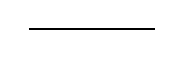
\begin{tikzpicture} 
					\draw[thick] (-0.8, 0) -- (0,0) -- (0.8, 0);
		\end{tikzpicture}}}
		+
		\vcenter{\hbox{\begin{tikzpicture} 
					\draw[thick,insert vertex=0] (0,0) arc(270:-90:0.4);
					\draw[thick] (-0.8, 0) -- (0,0) -- (0.8, 0);
		\end{tikzpicture}}}
		+
		\vcenter{\hbox{\begin{tikzpicture} 
					\draw[thick,insert vertex=0] (0,0) arc(270:-90:0.4);
					\draw[thick,insert vertex=0] (1,0) arc(270:-90:0.4);
					\draw[thick] (-0.8, 0) -- (1.8, 0);
		\end{tikzpicture}}}
		+ \dots &=
		\vcenter{\hbox{\begin{tikzpicture}
					\draw[insert vertex3=(0)](0,0);
					\draw[thick] (-1, 0) -- (1, 0);
		\end{tikzpicture}}} \; .
	\end{align}
Effectively, the resummation hence boils down to the substitution $m^2_\phi \rightarrow m^2_\phi + \Pi_\phi(T_\text{d})$ in $V_\text{T}(\phi, T_\text{d})$. In this thesis, we choose to use the Arnold-Espinoza method~\cite{Arnold:1992rz} for daisy resummation in which only the Matsubara-zero mode's contribution is resummed, as opposed to the Parwani method~\cite{Parwani:1991gq} or the full dressing procedure~\cite{Curtin:2016urg}, to spare the introduction of temperature-dependent counter terms. Algebraically, the resummation of the hard thermal loops can be achieved by the replacement~\cite{Carrington:1991hz} 
\begin{align}
	&\bb{V_\text{CW}+ V_\text{T}}_{m_\phi^2 \rightarrow m_\phi^2 + \Pi_\phi} = V_\text{CW} + V_\text{T} + V_\text{daisy} \nonumber \\
	&\text{with} \quad 
	V_{\text{daisy}}(\phi, T_\text{d}) = - \frac{T_\text{d}}{12 \pi} \bb{\ba{m^2_\phi + \Pi_\phi(T_\text{d})}^{3/2} - \ba{m^2_\phi}^{3/2}}
	\label{eq:daisy1}
\end{align}
The contributions from gauge bosons follow the same expression up to a factor for their internal \acp{dof}. As only longitudinal gauge bosons obtain Debye masses (see fig.~\ref{fig:hardthermalloops}), only the longitudinal \acp{dof} of a gauge boson need to be considered.

\paragraph{Summary} Summing all discussed terms together, we obtain the one-loop, daisy-resummed effective potential of the \ac{QFT} defined by the Lagrangian in eq.~\eqref{eq:toylagrangian}~\cite{Baker:2017zwx}
\begin{align}
	V_\text{eff}(\phi, T_\text{d}) = V_\text{tree} + V_\text{CW} + V_\text{ct} + V_T + V_\text{daisy}
	\label{eq:Veff}
\end{align}
with the individual contributions
	\begin{align}
		V_\text{CW}(\phi) &= \sum_{a = \phi, \varphi, A^\prime, \chi} \eta_a  n_a \frac{m_a^4(\phi)}{64 \pi^2} \bb{\ln \frac{m_x^2(\phi)}{v_\phi^2} - C_a} , \nonumber\\
		V_\text{T}(\phi, T_\text{d}) &= \frac{T^4}{2 \pi^2} \sum_{a = \phi, \varphi, A^\prime, \chi}  \eta_a n_a\ J_{\eta_a} \ba{\frac{m_a^2(\phi)}{T^2_\text{d}}} , \nonumber\\
		V_\text{daisy}(\phi, T_\text{d}) &= - \frac{T_\text{d}}{12 \pi} \sum_{b = \phi, \varphi, A_\text{L}^\prime} n_b \bb{\ba{m^2_b + \Pi_b(T_\text{d})}^{3/2} - \ba{m^2_b}^{3/2}}  \nonumber , \\
		V_\text{ct}(\phi) &= - \frac{\delta \mu^2}{2} \phi^2 + \frac{\delta \lambda}{4} \phi^4 \nonumber \\
		\text{with} & \quad \Pi_{\phi} = \Pi_{\varphi} = \left(\frac{\lambda}{3} + \frac{y^2}{12} + \frac{g^2}{4}\right)T^2_\text{d} \, , \quad 
		\Pi_{A'} = \frac{3}{4} g^2 T^2_\text{d} \, , \nonumber \\
		 &\quad  \delta \mu^2 = \left. \bb{\frac{3}{2 \phi} \td{V_\text{CW}(\phi)}{\phi} - \frac{1}{2} \tdd{V_\text{CW}(\phi)}{\phi}}\right|_{\phi = v_\phi}  , \nonumber \\
		\text{and}&\quad  \delta \lambda = \left. \bb{\frac{1}{2 \phi^3} \td{V_\text{CW}(\phi)}{\phi} - \frac{1}{2 \phi^2} \tdd{V_\text{CW}(\phi)}{\phi}}\right|_{\phi = v_\phi} . 
	\end{align}
As above, $n_a$ are the \acp{dof} of the fields coupled to $\phi$, $\eta_x$ is $+1$ ($-1$) for bosons (fermions), $C_a = 3/2 \ (5/6)$ are the renormalization constants for scalars and fermions (gauge bosons), and $J_{\eta_a}$ are the thermal functions as defined in eq.~\eqref{eq:thermalfunction}.

There have been developments in favor of a more rigorous calculation of the effective potential which allows for an expansion not in terms of the number of loops but in terms of powers of the coupling constants. This can be achieved through the construction of a three-dimensional effective field theory by formally integrating out the hard thermal scale (corresponding to the resummation of daisies), as well as the parameterically smaller soft and ultra-soft thermal scale (also resumming so-called super-daisies, lollipops and sunset diagrams)~\cite{Laine:2016hma,Curtin:2016urg}. The resulting \graffito{Super-daisies, lollipops and sunsets} effective potentials recovered through this procedure in particular do not suffer from a strong dependence of a specific chosen gauge and renormalization scale in contrast to the above calculation. Recently, dimensional reduction has become a feasible task using the Mathematica package \texttt{DRalgo}~\cite{Ekstedt:2022bff}. In chapter~\ref{chp:LISA} we use \texttt{DRalgo} in order to perform a cross-check and validate our results obtained using the effective potential from eq.~\eqref{eq:Veff}.


\section{Bubble nucleation and percolation}
\label{sec:fopts}

We are now well-equipped to study \acp{PT} in the early universe. To start with, let us study the derived effective potential in more detail: In fig.~\ref{fig:effpotential} we schematically plot $V_\eff(\phi, T_\text{d})$ for a range of temperatures given two benchmark points, one with $g = 0$ on the left-hand side and one with $g \neq 0$ on the right-hand side. At low temperature, in both cases the tree-level potential is recovered, having a minimum at the \ac{vev} $v_\phi$. At \graffito{A thermally induced barrier in $V_\mathrm{eff}$} sufficiently high temperatures, we further see that in both cases the minimum of the potential shifts to $\phi = 0$, which corresponds to the previously mentioned phenomenon of symmetry restoration. For intermediate temperatures, the effective potentials however are fundamentally different: For non-zero gauge couplings a thermally induced potential barrier is produced. 

\begin{figure}[t]
	\centering
	\includegraphics[width=\linewidth]{thesisplots/eff_pot/eff_potential}
	\caption{Sketch of the effective potential~\eqref{eq:Veff} corresponding to the Lagrangian in eq.~\eqref{eq:toylagrangian} for a set of decreasing temperatures (orange to blue curves). Left: $g = 0$, no potential barrier can form. Right: $g \neq 0$, a \ac{FOPT} can happen due to the generation of a potential barrier.}
	\label{fig:effpotential}
\end{figure}

The origin of this potential barrier can be traced down to the $z^3$ term in eq.~\eqref{eq:high-TJbos}, which only appears in the bosonic but not the fermionic thermal function. In fact, one can show that a thermally induced potential barrier can only be produced in the presence of transversal gauge bosons, as the daisy potential $V_\text{daisy}$ effectively cancels thermal barriers induced by \graffito{The barrier is due to transversal gauge bosons} loops of scalars and longitudinal gauge bosons: Expanding $V_\text{daisy}$ in the high-temperature regime, it evaluates to $T_\text{d}^4 \sum_b z^3_b /(12 \pi)$, such that after adding the $z_b^3$ piece of $V_\text{T}$ to it only the transversal gauge boson barrier survives.

In the presence of a potential barrier, the scalar field $\phi$ cannot smoothly transition to a new potential minimum, i.e.~$\phi$ cannot be homogeneous at all times. Instead, for temperatures below the critical temperature $T_\mathrm{d,c}$ at which the minima degenerate, bubbles of the new phase can nucleate, expand, accelerate up to relativistic velocities, and eventually \graffito{Below $T_\mathrm{d,c}$ bubbles can nucleate} collide, thereby possibly emitting strong gravitational radiation. In fig.~\ref{fig:bubbleexpansion} a sketch of the bubble nucleation can be found: A bubble's radius $r$, initially sufficiently large such that the bubble does not collapse under its own surface tension, will grow like $r  = \left|\mathbf{x}\right| = \sqrt{R^2 + c^2 t^2}$ if the interactions of the bubble wall with the plasma can be neglected~\cite{Linde:1980tt, Linde:1981zj}.

\begin{figure}[t]
	\myfloatalign
	\subfloat[]{
		\begin{tikzpicture}
			[
			dot/.style = {circle, fill, minimum size=#1, inner sep=0pt, outer sep=0pt, fill={rgb,255: red,0; green,159; blue,223}, text=white},
			dot/.default = 6pt,  % size of the circle diameter
			] 
			\node[dot=2.5cm](0) at (0,0) {$\phi \neq 0$};
			\node[above right = 0.3cm of 0] (1) {};
			\node[right = 0.3cm of 0] (2) {};
			\node[below right = 0.3cm of 0] (3) {};
			\node[below = 0.3cm of 0] (4) {};
			\node[below left = 0.3cm of 0] (5) {};
			\node[left = 0.3cm of 0] (6) {};
			\node[above left = 0.3cm of 0] (7) {};
			\node[above = 0.3cm of 0] (8) {};
			
			\draw [->, > = Triangle, draw={rgb,255: red,0; green,159; blue,223}, line width = 0.5mm] (0) to (1.center);
			\draw [->, > = Triangle, draw={rgb,255: red,0; green,159; blue,223}, line width = 0.5mm] (0) to (2.center);
			\draw [->, > = Triangle, draw={rgb,255: red,0; green,159; blue,223}, line width = 0.5mm] (0) to (3.center);
			\draw [->, > = Triangle, draw={rgb,255: red,0; green,159; blue,223}, line width = 0.5mm] (0) to (4.center);
			\draw [->, > = Triangle, draw={rgb,255: red,0; green,159; blue,223}, line width = 0.5mm] (0) to (5.center);
			\draw [->, > = Triangle, draw={rgb,255: red,0; green,159; blue,223}, line width = 0.5mm] (0) to (6.center);
			\draw [->, > = Triangle, draw={rgb,255: red,0; green,159; blue,223}, line width = 0.5mm] (0) to (7.center);
			\draw [->, > = Triangle, draw={rgb,255: red,0; green,159; blue,223}, line width = 0.5mm] (0) to (8.center);
			
			\node[dot=1.5cm](10) at (2.2,-2) {$\phi \neq 0$};
			\node[above right = 0.115cm of 10] (11) {};
			\node[right = 0.15cm of 10] (12) {};
			\node[below right = 0.15cm of 10] (13) {};
			\node[below = 0.15cm of 10] (14) {};
			\node[below left = 0.15cm of 10] (15) {};
			\node[left = 0.15cm of 10] (16) {};
			\node[above left = 0.15cm of 10] (17) {};
			\node[above = 0.15cm of 10] (18) {};
			
			\draw [->, > = Triangle, draw={rgb,255: red,0; green,159; blue,223}, line width = 0.3mm] (10) to (11.center);
			\draw [->, > = Triangle, draw={rgb,255: red,0; green,159; blue,223}, line width = 0.3mm] (10) to (12.center);
			\draw [->, > = Triangle, draw={rgb,255: red,0; green,159; blue,223}, line width = 0.3mm] (10) to (13.center);
			\draw [->, > = Triangle, draw={rgb,255: red,0; green,159; blue,223}, line width = 0.3mm] (10) to (14.center);
			\draw [->, > = Triangle, draw={rgb,255: red,0; green,159; blue,223}, line width = 0.3mm] (10) to (15.center);
			\draw [->, > = Triangle, draw={rgb,255: red,0; green,159; blue,223}, line width = 0.3mm] (10) to (16.center);
			\draw [->, > = Triangle, draw={rgb,255: red,0; green,159; blue,223}, line width = 0.3mm] (10) to (17.center);
			\draw [->, > = Triangle, draw={rgb,255: red,0; green,159; blue,223}, line width = 0.3mm] (10) to (18.center);
			
			\node at (-1,-2.5) {$\phi = 0$};
		\end{tikzpicture}
	} \quad
	\subfloat[]{\includegraphics[height=2.2in]{thesisplots/bubble_expansion/bubble_expansion}}
	\caption[]{\textit{Left}: Sketch of the bubble nucleation. Inside the bubbles $\phi \neq 0$, whereas the vacuum around them is still in the $\phi = 0$ phase. \textit{Right}: Sufficiently large bubbles can expand and accelerate up the speed of light.}
	\label{fig:bubbleexpansion}
\end{figure}

We now want to compute the temperature of the primordial plasma at which bubble nucleation happens. There are two different mechanisms through which the transition can be triggered: quantum tunneling and thermal fluctuations. We will only consider the case of \acp{PT} induced by thermal fluctuations, which typically have a bubble nucleation rate which exceeds that of tunneling-induced \graffito{The bubble nucleation rate} transitions except for the case of very strong supercooling~\cite{Athron:2023xlk}. In a semi-analytical approximation the bubble nucleation rate (per unit volume and time) reads~\cite{Coleman:1977py, Linde:1980tt, Linde:1981zj}
\begin{align}
	\Gamma(t) = A(T_\text{d}) \exp \bb{-\frac{S_3(T_\text{d})}{T_\text{d}}}, \label{eq:nuclrate}
\end{align}
where $S_3(T_\text{d})$ is referred to as the (Euclidean) bounce action. The latter is given by 
\begin{align}
	S_3\ba{T_\text{d}} \equiv S_3\bb{\phi_\text{b}(\bm{x}; T_\text{d})} =  \int \diff^3 x \bb{ \frac{\ba{\nabla \phi_\text{b}}^2}{2} + V_\text{eff}(\phi_\text{b}, T_\text{d})} \, 
\end{align}
where $\phi_\text{b}(\bm{x}; T_\text{d})$ is the ``bounce'' solution of the $O(3)$-symmetric Klein-Gordon equation
\begin{align}
	\pdd{\phi}{r} + \frac{2}{r} \pd{\phi}{r} = \td{V_{\text{eff}}(\phi, T_\text{d}) }{\phi} \equiv V_{\text{eff}}^\prime(\phi, T_\text{d}) \, .
\end{align}
Here, we made the bubble's $O(3)$ symmetry manifest by choosing spherical coordinates with $r = \abs{\bm{x}}$ denoting the distance to the bubble center. The latter Klein-Gordon equation interpolates $\phi(r)$ between the two phases and hence determines the bubble profile $\phi_\text{b}(r; T_\text{d})$. To determine it numerically given a potential $V_\text{eff}$, we impose the boundary conditions $\phi(r \rightarrow \infty )  \rightarrow 0$ and $\phi^\prime(r = 0) = 0$ and use a shooting algorithm (see fig.~11 in ref.~\cite{Athron:2023xlk}).

The time-dependence in eq.~\eqref{eq:nuclrate} was reintroduced to indicate that $T_\text{d}(t)$ is a dynamical quantity due to the Hubble expansion. Note that previously we assumed that there are no dynamical processes such that we could work in the imaginary time formalism to derive $V_\text{eff}(\phi, T_\text{d})$. \graffito{The reappearance of dynamics} This assumption still holds very well in the limit of a sufficiently slow Hubble expansion. This assumption can be checked explicitly by comparing typical particle interaction rates with the Hubble rate (cf.~chapter~\ref{sec:thermalization}).

In fig.~\ref{fig:phases} a schematic overview of the different quantities going into the calculation of the bubble nucleation rate is shown: From a given effective potential the phase structure can be obtained by tracking the position of the potential minima over a range of temperatures. If there exists an overlap in which two phases separated by a potential barrier coexist, a \ac{FOPT} can occur. The bubble profile of an expanding bubble is shown on the \graffito{The bubble profile} right: Within the bubble, at $r<\sqrt{R^2 + t^2}$, where $R$ is the initial bubble radius and $t$ is the time passed since the individual bubble's nucleation, the scalar field obtains the \ac{vev} of the true minimum. In front of the bubble wall, the field quickly goes to the false vacuum's \ac{vev}. Note that there is some temperature dependence of the true minimum's \ac{vev} as can be seen in the light blue curve in the left panel, which we refer to $\phi_\text{max}$ in the right panel.

\begin{figure}[t]
	\centering
	\includegraphics[width=\linewidth]{thesisplots/phases/phases}
	\caption{
		\textit{Left}: The coexistence of potential minima in range of temperatures allows for a \ac{FOPT} which succeeds through the nucleation of bubbles at $T_\text{n}$. \textit{Right}: A bubble profile which interpolates between the vacuum states on both sides of the bubble wall at $\sqrt{R^2 + t^2}$.
		}
	\label{fig:phases}
\end{figure}

We define the point in time at which nucleation happens by requiring that one bubble per Hubble patch has been produced. By dimensional analysis and for simplicity the prefactor of the nucleation rate can be approximated as $A(T_\mathrm{d}) \sim T_\mathrm{d}^4$. This is usually sufficient for leading-order calculations due to the exponential dependence of the bounce action. For a more rigorous and already automated calculation of $A(T_\text{d})$ up to one-loop order see for instance ref.~\cite{Ekstedt:2023sqc}. The number of \graffito{Nucleation happens when $S_3(T_\mathrm{d}) / T_\mathrm{d} \simeq \mathcal{O}(150)$} bubbles per Hubble patch can be calculated by integrating $\Gamma(t)$ over time. Due to the exponential time dependence, this integral can be well approximated by only considering the lowest temperature at which $\Gamma$ is evaluated, i.e.~the nucleation temperature. In doing so we immediately obtain the nulceation condition $\left. \Gamma H^{-4}\right|_{t_\text{n}} = 1$, which can be rewritten as~\cite{Caprini:2015zlo}
\begin{align}
	\left.\frac{S_3(T_\text{d})}{T_\text{d}}\right|_{T_\text{d,n} = \xi_\text{n} T_\text{n}} \simeq 146 - 2 \ln \ba{\frac{g_{*}(T_\text{n})}{100}} - 4 \ln \ba{\frac{T_\text{n}}{100 \, \text{GeV}}}
	\label{eq:nuclcrit}
\end{align}
upon plugging in the Hubble rate $H^2(T) = \frac{\pi^2}{90} g_*(T) T^4/\Mp^2$ in radiation domination. In summary, nucleation is expected to happen when $S_3/T_\text{d}$ crosses $\log(\Mp^4/T_\text{n}^4) \simeq \mathcal{O}(150)$. Numerically, the nucleation temperature can hence be found iteratively by repeated evaluation of the above nucleation condition at different temperatures. Note that the above criterion is only approximate and needs to be corrected in case the amount of vacuum energy in the \ac{DS} is so large that it leads to a second inflationary period, breaking the assumption of radiation domination. 

In fig.~\ref{fig:nuclcrit} we schematically show how the bounce action drops for a decreasing \ac{DS} temperature. Note that at $T_\text{d,c}$ when the two minima are at the same vacuum energy such that $\Delta V_\text{eff} = 0$, the bounce action diverges and the bubble nucleation rate hence drops to zero, corresponding to a zero probability for the nucleation of a bubble at a given point in space.

\begin{figure}[t]
	\centering
	\includegraphics[width=\linewidth]{thesisplots/nuclcrit/nuclcrit}
	\caption{
		The temperature dependence of the bounce action $S_3(T_\text{d}) / T_\text{d}$ over a range of temperatures. At {\color{DESYdunkelrot} $T_\text{d,c}$} the bounce  action diverges since $\Delta V_\text{eff} = 0$, corresponding to a vanishing bubble nucleation rate. At {\color{DESYorange} $T_\text{d,n}$} the bounce action becomes low enough for the nucleation of one bubble per Hubble volume. Percolation happens at {\color{DESYgelb} $T_\text{d,p}$}.}
	\label{fig:nuclcrit}
\end{figure}

Bubble nucleation alone is not sufficient for the completion of a \ac{PT}. In case of a strongly super-cooled \ac{PT}, i.e.~for a large difference in vacuum energy between the two phases, the Hubble parameter can be dominated by $\Delta V_\text{eff}$ leading to an exponential growth of the scale factor, forbidding the collision of bubbles. It therefore makes sense to check \graffito{Percolation} whether at some point in time the new phase actually percolates the universe by a connected web of bubbles~\cite{Guo:2021qcq, Athron:2023rfq,Caprini:2019egz}. This point in time is specified by roughly 30\% of the Hubble volume having transitioned to the true vacuum state. The corresponding false-vacuum fraction is given by $P(T) = \exp \bb{-I(T)}$ with~\cite{Athron:2023xlk}
\begin{align}
	I(T) = \frac{4 \pi}{3} \vw^3 \int^{T_\text{c}}_{T} \diff T^\prime  \frac{\Gamma(T^\prime)}{T^{\prime\,4} \, H(T^\prime) } \ba{\int_{T}^{T^\prime}  \frac{\diff T^{\prime\prime}}{H(T^{\prime\prime})}}^3 , \label{eq:falsvacfrac}
\end{align}
where $\vw$ is the terminal bubble wall velocity resulting from interactions of the bubble wall with the surrounding plasma. The resulting percolation temperature $T_\text{p} \lesssim T_\text{n}$, which can be determined from the condition $I(T_\text{p}) = 0.34$, approaches the nucleation temperature $T_\text{n}$ in the limit of weak \acp{PT}, but can be orders of magnitude smaller in the case of strong super-cooling~\cite{Ellis:2018mja}.

\section{Gravitational waves from dark sector phase transitions} \label{sec:gwfopt}

In principle, we now have all the necessary ingredients to predict the \ac{GWB} emitted during a \ac{FOPT}. In practice, this is typically achieved by simulating the nucleation, expansion, and collision of bubbles on a lattice. This approach allows us to access the anisotropic stress within the perturbed plasma, and thereby the \ac{GW} spectrum that emerges over time~\cite{Hindmarsh:2020hop}. However, bubble expansion is complicated by the feedback from fluid dynamics, making these computations increasingly demanding depending on the size of the simulated volume and the chosen grid spacing. \graffito{Lattice simulations are expensive} To accurately approximate the generated \ac{GW} signal, the simulated volume should include as many bubbles as possible, and the grid spacing must be smaller than the relevant scales to precisely model the fluid dynamics. Additionally, the bulk fluid motion that sources \acp{GW} can persist much longer than the bubble collisions themselves~\cite{Caprini:2019egz}, necessitating long simulation times. As a result, predicting the \ac{GW} spectrum for a specific transition in a given effective potential is computationally too expensive to simulate in each case. Fortunately, there are widely used approximations derived from a combination of analytical and numerical methods that can effectively predict \ac{GWB} spectra. We will now discuss how to map a given effective potential to these semi-analytical expressions.

To do so, let us introduce a set of useful dimensionless parameters which characterize the thermodynamics of \acp{DSPT}: The most relevant parameters for the calculation of the \ac{GWB} spectrum, next to the previously derived percolation temperature $T_\text{p}$, are the strength parameters $\alpha$ and $\alpha_\text{DS}$ and the speed $\beta/H$ of the \ac{PT}.

The strength parameter $\alpha$  quantifies the amount of latent heat released in the \ac{PT} and relates it to the total energy density $\rho_\text{SM}^\perc + \rho_\text{DS}^\perc$ of both the \ac{DS} and the \ac{SM} bath at the time of percolation.  In ref.~\cite{Hindmarsh:2015qta}, the trace $\theta_\text{d} \equiv - \eta_{\mu \nu} T^{\mu \nu}_\text{d} = - 4  V_\text{eff} + T_\text{d} \pd{V_\text{eff}}{T_\text{d}}$ of the \graffito{The transition strength} \ac{DS}'s energy momentum tensor $T^\mn_\text{d}$ has been advertised to be a good parameterization for mapping between a given effective potential to the performed numerical simulations. The effective potential is here understood to be evaluated at the percolation temperature $T_\text{d,p}$. The latent heat can then be obtained through $\Delta \theta_\text{d}/4$, where $\Delta$ refers to a difference between the two phases. The strength of the phase transition can hence be expressed as
\begin{align}
	\alpha \equiv \frac{\Delta \theta_\text{d} / 4}{\rho_\text{SM}^\text{p} +\rho_\text{DS}^\text{p}}  && \text{with} && \Delta \theta_\text{d} = \bb{ - 4 \Delta V_\text{eff} + T_\text{d} \pd{\Delta V_\text{eff}}{T_\text{d}} }_{T_{\text{d,p}}}  > 0 \, ,
	\label{eq:alpha}
\end{align}
where $\Delta V_\text{eff}$ denotes the potential difference between the two vacua. This parameterization of $\alpha$ has become a useful standard as it does not suffer from the inaccuracies which arise when using the pressure or vacuum energy difference instead of the trace difference $\Delta \theta_\text{d}$, as advertised in earlier works~\cite{Athron:2020maw, Giese:2020rtr}. 

In case the \ac{DS} is completely secluded, there is another important transition \graffito{Dark bubble walls only feel the \ac{DS}} strength parameter: It can be obtained by instead normalizing $\Delta \theta_\text{d}$ to the \ac{DS} energy density alone~\cite{Ertas:2021xeh, Bringmann:2023opz}, 
\begin{align}
	\alpha_\text{DS} \equiv \frac{\Delta \theta_\text{d}/4}{\rho_\text{DS}^\text{p}} = \alpha \ba{1 + \frac{1}{\xi_\text{p}^4 } \frac{g_\SM(T_\text{p})}{g_\DS(T_\text{p})}} \, , \label{eq:alphaDS}
\end{align}
where $\xi_\text{p} = T_\text{d,p}/T_\text{p}$ is the temperature ratio the between symmetric phase of the \ac{DS} and the \ac{SM} bath at the time of percolation. In a \ac{DSPT}, the bubble wall can only feel the effect of \ac{DS} states, as visible sector states do not obtain masses throughout the transition. The percentage of liberated vacuum energy density available for accelerating the bubble wall will hence depend on $\alpha_\text{DS}$ and not on $\alpha$. This is an important difference with respect to the case of visible sector \acp{PT}. Also quantitatively, the difference between $\alpha_\text{DS}$ and $\alpha$ can be enormous due to the factor $\xi_\text{p}^4$. The temperature ratio $\xi_\text{p}$ therefore strongly impacts the dynamics of the dark bubble walls. 

The speed of the \ac{PT} expressed in units of the Hubble rate at the time of percolation can be determined by calculating \graffito{The transition speed} the slope of the bounce action at $T_\text{p}$,
\begin{align}
	\beta/H \equiv \left. \frac{1}{H} \td{\log \Gamma}{t} \right|_{t_\text{p}} \simeq T_{\text{d,p}} \left. \frac{\diff}{\diff T_\text{d}}  \frac{S_3(T_\text{d})}{T_\text{d}} \right|_{T_\text{d,p}} \, . \label{eq:betaH}
\end{align}
Typically, $S_3 / T_\text{d}$ can be expanded as a polynomial in $T_\text{d}$ around $T_\text{d,p}$, such that $\beta/H = \mathcal{O} \ba{{S_3(T_\text{d,p}) / T_\text{d,p}}}$.
As we argued in eq.~\eqref{eq:nuclcrit}, nucleation happens when $S_3(T_\text{d,n})/T_\text{d,n} = \mathcal{O}(150)$. For sufficiently weak phase transitions $T_\text{d,p} \simeq T_\text{d,n}$ holds. Quite generally, one can hence expect $\beta/H \simeq \mathcal{O}(100-1000)$ depending on the strength of the \ac{PT}~\cite{Bringmann:2023opz}. Obtaining smaller values for $\beta/H$, in order to produce stronger \ac{GW} signals, is possible for near-conformal potentials~\cite{Randall:2006py, Konstandin:2011dr, Ellis:2020nnr, Kierkla:2022odc, vonHarling:2017yew, Bruggisser:2018mrt, Bruggisser:2022rdm, Baldes:2021aph} or at the expense of tuning the scalar potential such that the system is close to meta-stable (if it does not tunnel during the lifetime of the Universe). For as small values as $\beta/H=\mathcal{O}(1)$, however, the phase transition might not complete and a phase of eternal inflation might occur~\cite{Randall:2006py, Konstandin:2011dr, vonHarling:2017yew, Bruggisser:2018mrt, Bruggisser:2022rdm, Baldes:2021aph, Athron:2023xlk}.

Typically, a \ac{PT} is referred to as \textit{strong} when $\alpha \gtrsim \mathcal{O}(1)$ and \textit{slow} when $\beta/H \lesssim \mathcal{O}(100)$. Both conditions need to be fulfilled in order to obtain observable \ac{GW} signals as we will see in the following section. This corresponds to a latent heat release $\Delta V_\text{eff} \simeq \rho_\text{SM}^\text{p} + \rho_\text{DS}^\text{p}  $ of \graffito{Strong and slow relative to what?} the order of the energy density of the primordial plasma before the transition and a duration of the transition $\beta^{-1}$ of at least a hundredth of a Hubble time. To give some meaning to these scales, let us consider a \ac{PT} percolating at a $100 \, \text{MeV}$ temperature for preciseness: Requiring it to be slow and strong according to the above criteria implies a minimum duration on the µs scale and a released equivalent mass density of roughly $10^{14} \, \text{g} \, \text{cm}^{-3}$ respectively. The latter is approximately the mass density of a neutron star. Due to the sheer size of the expected energy flows, we can hence expect the emission of observable \acp{GWB} by such transitions.

\subsection{Bubble collisions and sound waves}
\label{sec:bwsw}

The \ac{GW} spectrum emitted in \acp{FOPT} is sourced by a set of intertwined physical processes, most importantly bubble collisions, as well as sound waves and turbulence in the perturbed plasma. Each of these contributions can potentially dominate the \ac{GW} spectrum, depending in particular on the speed $\vw$ of the bubble wall and the strength $\alpha_\text{DS}$ of the \ac{PT}. Since predictions for plasma turbulence as a \ac{GW} source often requires especially long lattice simulations with small grid spacing~\cite{RoperPol:2019wvy}, which are not yet understood well enough to make \graffito{The energy budget of a \ac{PT}} quantitative statements~\cite{Caprini:2019egz}, we will only consider sound wave and bubble collision contributions in this thesis. The energy budget of a \ac{PT} is conventionally parameterized by the sum $\kappa_\phi + \kappa_\text{sw} + \kappa_\text{therm} = 1$, where the first contribution quantifies the percentage of liberated vacuum energy going into gradient field energy in the bubble walls, the second term corresponds to bulk fluid motion and $\kappa_\text{term}$ corresponds to an immediate increase of the thermal energy. In this thesis, we will work in the high-$\vw$ approximation discussed in the appendix of ref.~\cite{Espinosa:2010hh} in which $\kappa_\text{therm} \rightarrow 0$. We use the expression provided there to compute the efficiency $\kappa_\text{sw}$ in dependence of $\alpha_\text{DS}$. In section~\ref{app:darkwalls} we will discuss the validity of the high-$\vw$ approximation in the $U(1)^\prime$ model.

\paragraph{Bubble wall contributions}
The spectrum of \acp{GW} emitted by bubble collisions was first derived analytically and then studied in simulations using the so-called envelope approximation~\cite{Kamionkowski:1993fg, Kosowsky:1992vn, Kosowsky:1991ua}, in which a thin sheet with large gradient field energy around the collided bubbles is assumed to give rise to the anisotropic stress necessary for emitting \acp{GW}. Since then several analytical works~\cite{Jinno:2016vai, Caprini:2007xq, Huber:2008hg, Weir:2016tov, Konstandin:2017sat} have been performed in order \graffito{The envelope approximation} to refine the original results for the contribution of bubble wall collisions. In this thesis we will use the parameterization used in the \ac{LISA} 2015 review~\cite{Caprini:2015zlo} based on ref.~\cite{Huber:2008hg},
\begin{align}
	h^2 \Omega_\text{bw}(f) &= \mathcal{R}h^2 \, \tilde{\Omega}_\bw \,  \ba{\frac{\kappa_\phi\, \alpha}{\alpha + 1}}^2 \, \ba{\frac{\beta}{H}}^{-2} \, s_\bw(f/f_\text{p,\bw}) \nonumber \\
	\text{with} \quad s_\bw(x) &= \frac{3.8 x^{2.8}}{1 + 2.8 x^{3.8}} \qquad \text{and} \qquad f^\text{em}_\text{p,bw} / \beta = 0.23 \, . \label{eq:bw}
\end{align}
The amplitude of the signal at the time of production is fixed by $\tilde{\Omega}_\text{bw} = {0.11 \vw^3} / \ba{0.42 + \vw^2} = 0.077$ for $\vw \rightarrow 1$. Assuming entropy conservation between the spectrum's emission and today, the amplitude redshift $\mathcal{R}h^2$ follows the previously derived eq.~\eqref{eq:Rh2simple} and a given mode's frequency $f$ today is related to an emitted frequency $f^\text{em}$ through eq.~\eqref{eq:fredshiftsimple} with $x_k/(2 \pi)$ corresponding to the above expression for the spectrum's peak frequency at the time of emission $f_\text{p,bw}^\text{em}$. We see that the \ac{IR} slope of the spectrum $s_\text{bw}$ increases with $f^{2.8}$ (which is close to the causality \ac{IR} tail with $f^3$~\cite{Durrer:2003ja, Caprini:2009fx, Cai:2019cdl, Hook:2020phx}), whereas the \ac{UV} slope decreases slowly with $f^{-1}$.

Numerical \graffito{The bulk-flow model} simulations of bubble collisions lately challenged the envelope approximation: The peak frequency showed to be a factor 5 higher than previously expected and that the \ac{UV} slope should fall off more quickly with $f^{-1.5}$~\cite{Cutting:2018tjt}. In ref.~\cite{Cutting:2020nla} it was further shown that both the \ac{IR} and \ac{UV} slopes depend on the finite thickness of the wall profile, confirming previous analytical works~\cite{Jinno:2017fby, Konstandin:2017sat} referred to as the bulk-flow model. A concise comparison of the different parameterizations of the bubble wall spectrum can be found in chapter 6 of ref.~\cite{Gouttenoire:2022gwi}.

In a given particle physics model featuring a \ac{FOPT} the contribution from bubble wall collisions is, however, \graffito{Sound waves typically dominate} often expected to be subdominant compared to the contribution from sound shell collisions since $\kappa_\phi \ll \kappa_\text{sw}$. Only in the case of bubble walls which run away, i.e. if the bubble walls accelerate up to the point of their collision, the dominant contribution to the total \ac{GW} signal is expected to arise from bubble collisions~\cite{Vanvlasselaer:2022fqf}. 

\paragraph{Sound wave contributions}

The sound wave contributions to the total \ac{GWB} spectrum were first studied in the early 90s~\cite{Kamionkowski:1993fg}. Today, hydrodynamical simulations~\cite{Hindmarsh:2013xza, Hindmarsh:2015qta, Giblin:2014qia, Cutting:2019zws, Hindmarsh:2017gnf} and corresponding analytical investigations~\cite{Hindmarsh:2016lnk, Hindmarsh:2019phv} referred to as the sound shell model sustain the parameterization of the \ac{GWB} signal \graffito{The \ac{LISA} sound wave template} employed in the LISA 2019 review~\cite{Caprini:2019egz, Hindmarsh:2017gnf}, which we will also use in this thesis. It reads
\begin{align}
	h^2 \Omega_\text{sw}(f) &= \mathcal{R}h^2 \tilde{\Omega}_\sw  \ba{\frac{\kappa_\sw  \alpha}{\alpha + 1}}^2   \ba{\frac{\beta}{H}}^{-1}  \mathcal{Y}_\text{sh}  s_\sw(f/f_\text{p,\sw}) \nonumber \\
	\text{with} \quad s_\sw(x) &= x^3 \ba{\frac{7}{4 + 3 \, x^2}}^{7/2} \, , \qquad f^\text{em}_\text{p,sw} / \beta = 0.53 \nonumber  \\
	\text{and} \quad \mathcal{Y}_\text{sh} &= \min \bb{1, \tau_\text{sh} H} \simeq \min \bb{1, \frac{3.38}{\beta/H} \sqrt{\frac{1 + \alpha}{\kappa_\sw \alpha}}} \, . \label{eq:sw}
\end{align}
The normalization of the signal is given by $\tilde{\Omega}_\sw = 3 \times 0.012 \times 0.687 \times (8\pi)^{1/3} = 0.072$, where the first two factors were identified in ref.~\cite{Hindmarsh:2017gnf}, the third one arises from the normalization of the spectrum $\int s_\text{sw} \diff \log x  = 1/0.687$ and the fourth one converts the estimated mean bubble separations to $\beta/H$. Note that the initial factor 3 was erroneously missing in LISA 2019 review~\cite{Caprini:2019egz}. It should be noted that that this expression can lead to a slight overestimation of the \ac{GW} signal for sources being active for about a Hubble time. As the onset of turbulence is however an unsolved and model-dependent question, we conservatively stick to the shown expression for $\mathcal{Y}_\text{sh}$ despite the developments shown in ref.~\cite{Guo:2020grp}.

Depending on the strength $\alpha_\text{DS}$ and the bubble wall velocity $\vw$, either a shock wave forms in front or behind the bubble walls. These cases correspond to sub- and supersonic bubble wall velocities, referred to as deflagration and detonation fluid profiles, respectively. In this thesis, \graffito{The energy budget for fluid motion} we will use the fitting formula for $\vw \rightarrow 1$ provided in the appendix of ref.~\cite{Espinosa:2010hh} to calculate the efficiency $\kappa_\text{sw}$ for converting vacuum energy to bulk fluid motion. The factor $\mathcal{Y}_\text{sh}$ accounts for the lifetime $\tau_\text{sh}$ of the sound wave source, after which shocks form and non-linearities develop. Note that the sound wave contribution is only suppressed by a single power in $\beta/H$, whereas the bubble wall collision contributions scales with $\ba{\beta/H}^{-2}$. Typically the bubble wall contribution is therefore suppressed even for similar energy budgets $\kappa_\phi$ and $\kappa_\text{sw}$. 


\subsection{The dilution of GWs due to a dark sector decay} \label{sec:DSdecaydilution}

So far we did not specify any couplings to \ac{SM} states. As noted above, sufficiently small couplings (for instance to the \ac{SM} photon through kinetic mixing or to the \ac{SM} Higgs field through mass mixing) do not change the dynamics of the \ac{PT} as their effect on the effective potential can be neglected. A \ac{PT} in a secluded \ac{DS}, which cannot dispose of the liberated vacuum energy density, is subject to strong constraints due to the aforementioned $\DNeff$ constraints (cf.~eq.~\eqref{eq:DNeff}). We investigate \graffito{A decaying \ac{DS} can dilute the $\acp{GW}$} these constraints in detail in chapter~\ref{chp:ptabbn}. In previous studies it was realized that a decay of the \ac{DS} can circumvent these constraints at the cost of potentially changing the expansion history of the universe, especially if the \ac{DS} is hotter than the \ac{SM} bath and decays out-of-equilibrium~\cite{Ertas:2021xeh}. The effect of the resulting entropy injection into the \ac{SM} bath is an extra redshift between the time of \ac{GWB} emission and today with respect to the naive \ac{LCDM} expansion history. We refer to this additional decrease of the \ac{GWB} amplitude and peak frequency as dilution~\cite{Cirelli:2018iax}. It is characterized by the dilution factor
\begin{align}
	D \equiv \frac{S_\mathrm{SM}^{0}}{S_\mathrm{tot}^\mathrm{p}} \, ,
\end{align}
which relates the comoving entropy density of both the \ac{DS} and \ac{SM} \graffito{The effect of an entropy injection on $\mathcal{R}h^2$ and the peak frequency}  bath at the time of the \ac{PT} with the current comoving entropy density of \ac{SM} states. In case the \ac{DS} thermalizes with the \ac{SM} particles through the decay of a relativistic \ac{DS} state, $D \rightarrow 1$ and the effect on the redshift of the \ac{GW} signal is negligible. If instead a large amount of entropy is produced and injected into the \ac{SM} bath, the previous expression for the frequency redshift $f/f^\text{em}$ and amplitude redshift $\mathcal{R}h^2$ need to be corrected to~\cite{Ertas:2021xeh}
\begin{subequations}
	\label{eq:dilution}
	\begin{align}
		&f_{\text{p},i} = \frac{17 \, \text{nHz}}{D^{1/3}} \ba{\frac{\beta}{H}}  \ba{\frac{T_\text{p}}{100 \, \text{MeV}}} \ba{\frac{f_{\text{p},i}^\text{em}}{\beta}}  \ba{\frac{g_{\text{tot}}^\text{p}}{100}}^{1/2} \ba{\frac{100}{h_{\text{tot}}^\text{p}}}^{1/3}  \\
		&\text{and} 	\qquad \mathcal{R} h^2 = \frac{1.7 \cdot 10^{-5}}{D^{4/3}} \ba{\frac{g_{\text{tot}}^\text{p}}{100}} \ba{\frac{100}{h_{\text{tot}}^\text{p}}}^{4/3} \,. 
	\end{align}
\end{subequations}
The temperature $T_\text{p}$ here corresponds to the \ac{SM} bath at the time of percolation, at which also the \acp{dof} $g_\text{tot}^\text{p}$ and $h_\text{tot}^\text{p}$ of the combined bath of \ac{SM} and \ac{DS} particles are evaluated, cf.~eqs.~\eqref{eq:gstar} and~\eqref{eq:hstar}.